\documentclass{beamer}
\usetheme{metropolis}           % Use metropolis theme
%\usepackage[german]{babel}  
\usepackage[utf8]{inputenc}	%dt Sonderzeichen wie ß
\usepackage{tikz}
\usepackage{amssymb}
\usepackage{multirow}
\usepackage{pgfpages}
\usepackage{cite}
\usepackage{graphicx}
\usepackage{animate}


\usepackage{multimedia}
\usepackage{float}
\usepackage{subfig}
\usepackage{svg}
\usepackage{enumitem}


%\setbeameroption{show notes on second screen=right}  %% Uncomment this to get Notes


%\renewcommand*{\figurename}{Abb.}




\title{A configurable speech recognition pipeline for social robots}
\subtitle{Creating a fusion framework for analyzing speech data}
\date{4.7.2019}
\institute{Master Thesis}
\author{Robert Feldhans}
\begin{document}
	\maketitle
	
	\begin{frame}{Content}
		\setbeamertemplate{section in toc}[sections numbered]
		\tableofcontents[hideallsubsections]
	\end{frame}
	
	\section{Motivation}
	

	
	\begin{frame}{Foray Robocup Speechrec Task}
		\centering
		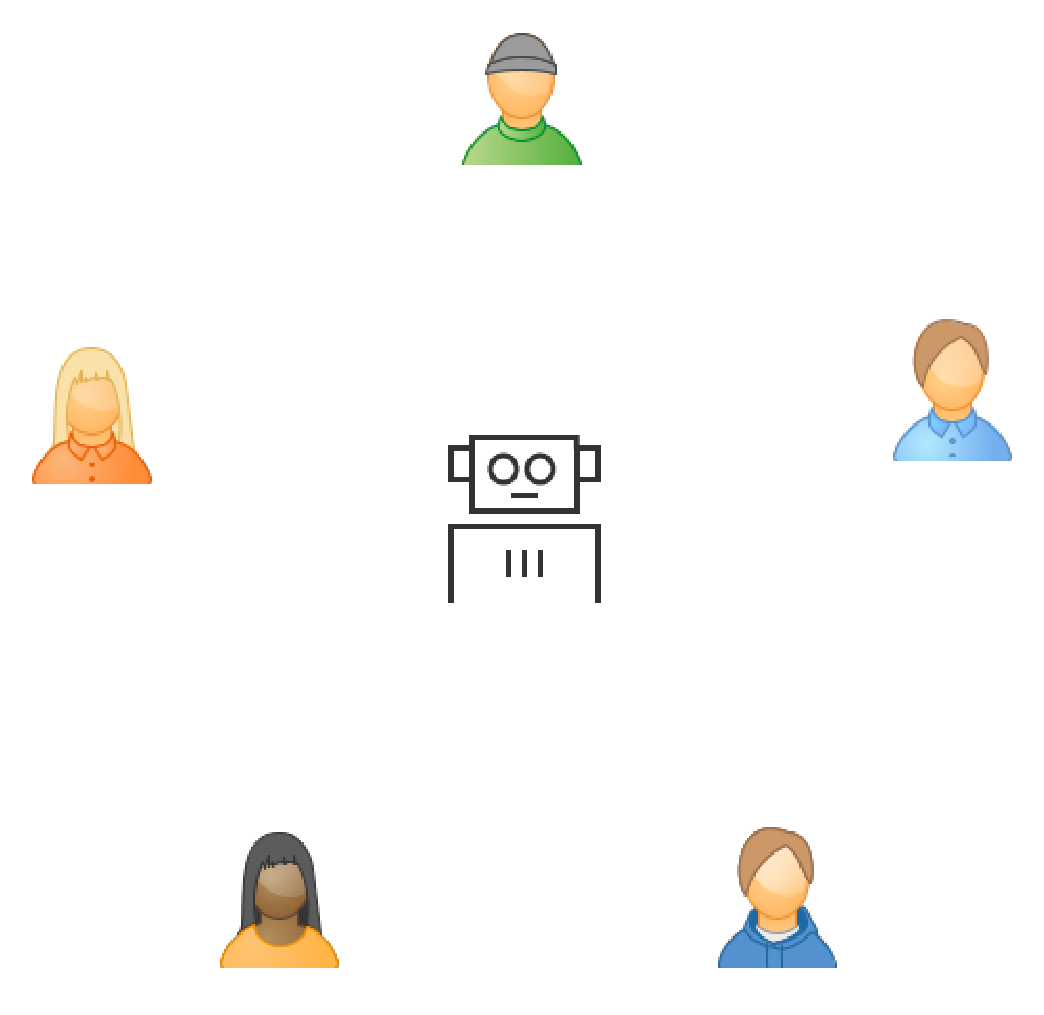
\includegraphics[width=.75\textwidth]{Bilder/robocup_task}
	\end{frame}
	
	\begin{frame}{Foray Robocup Speechrec Task}
		\centering
		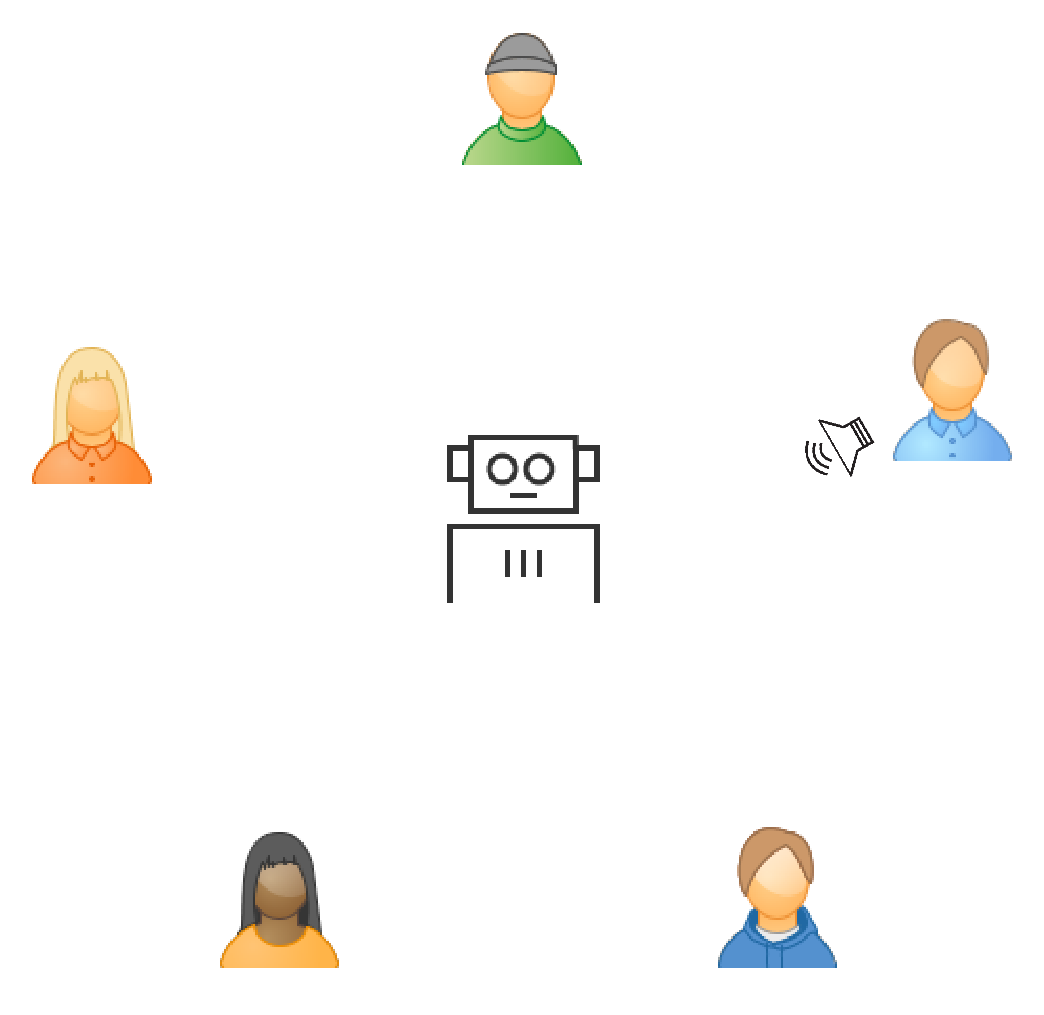
\includegraphics[width=.75\textwidth]{Bilder/robocup_task_1}
	\end{frame}
	
	\begin{frame}{Foray Robocup Speechrec Task}
		\centering
		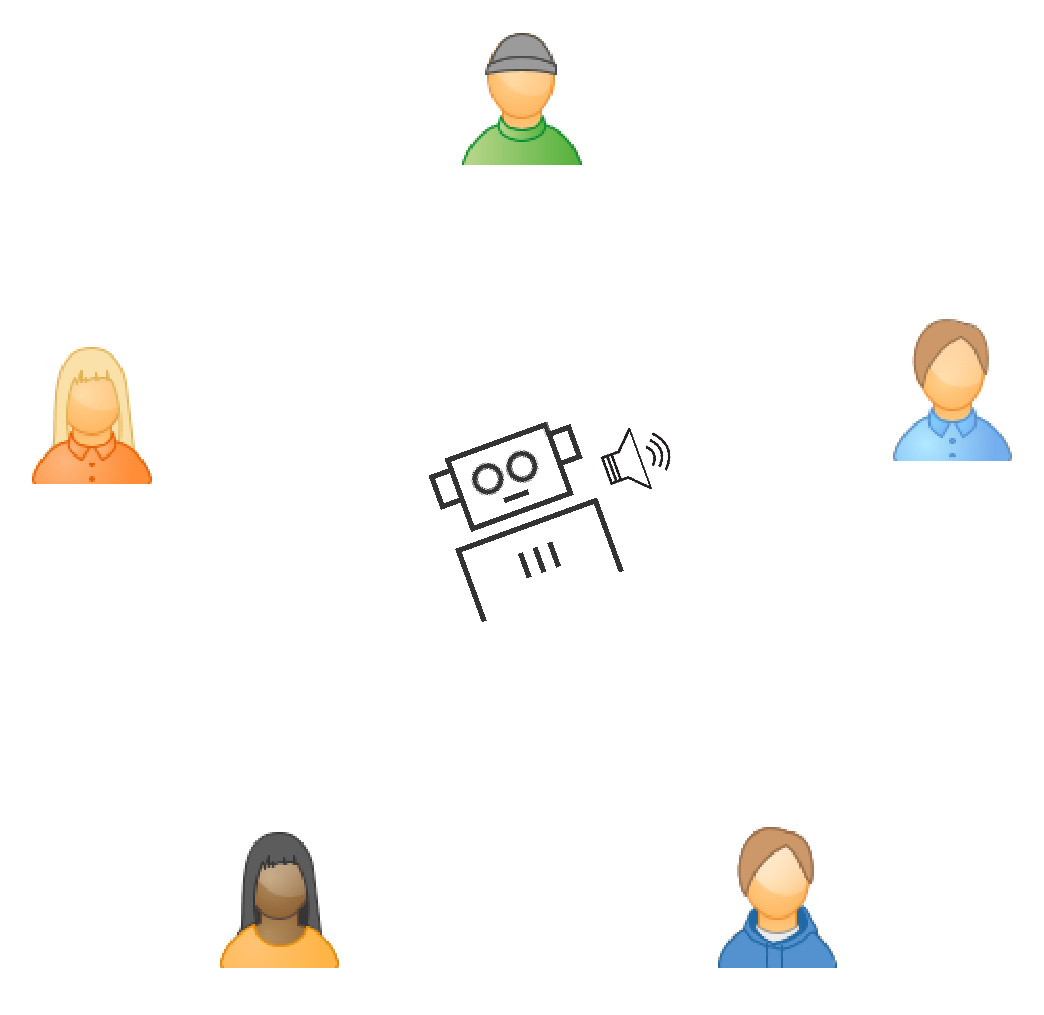
\includegraphics[width=.75\textwidth]{Bilder/robocup_task_2}
	\end{frame}
	
	\begin{frame}{Foray Robocup II}
		\centering
		\movie[width=\textwidth,poster,autostart,showcontrols,loop]{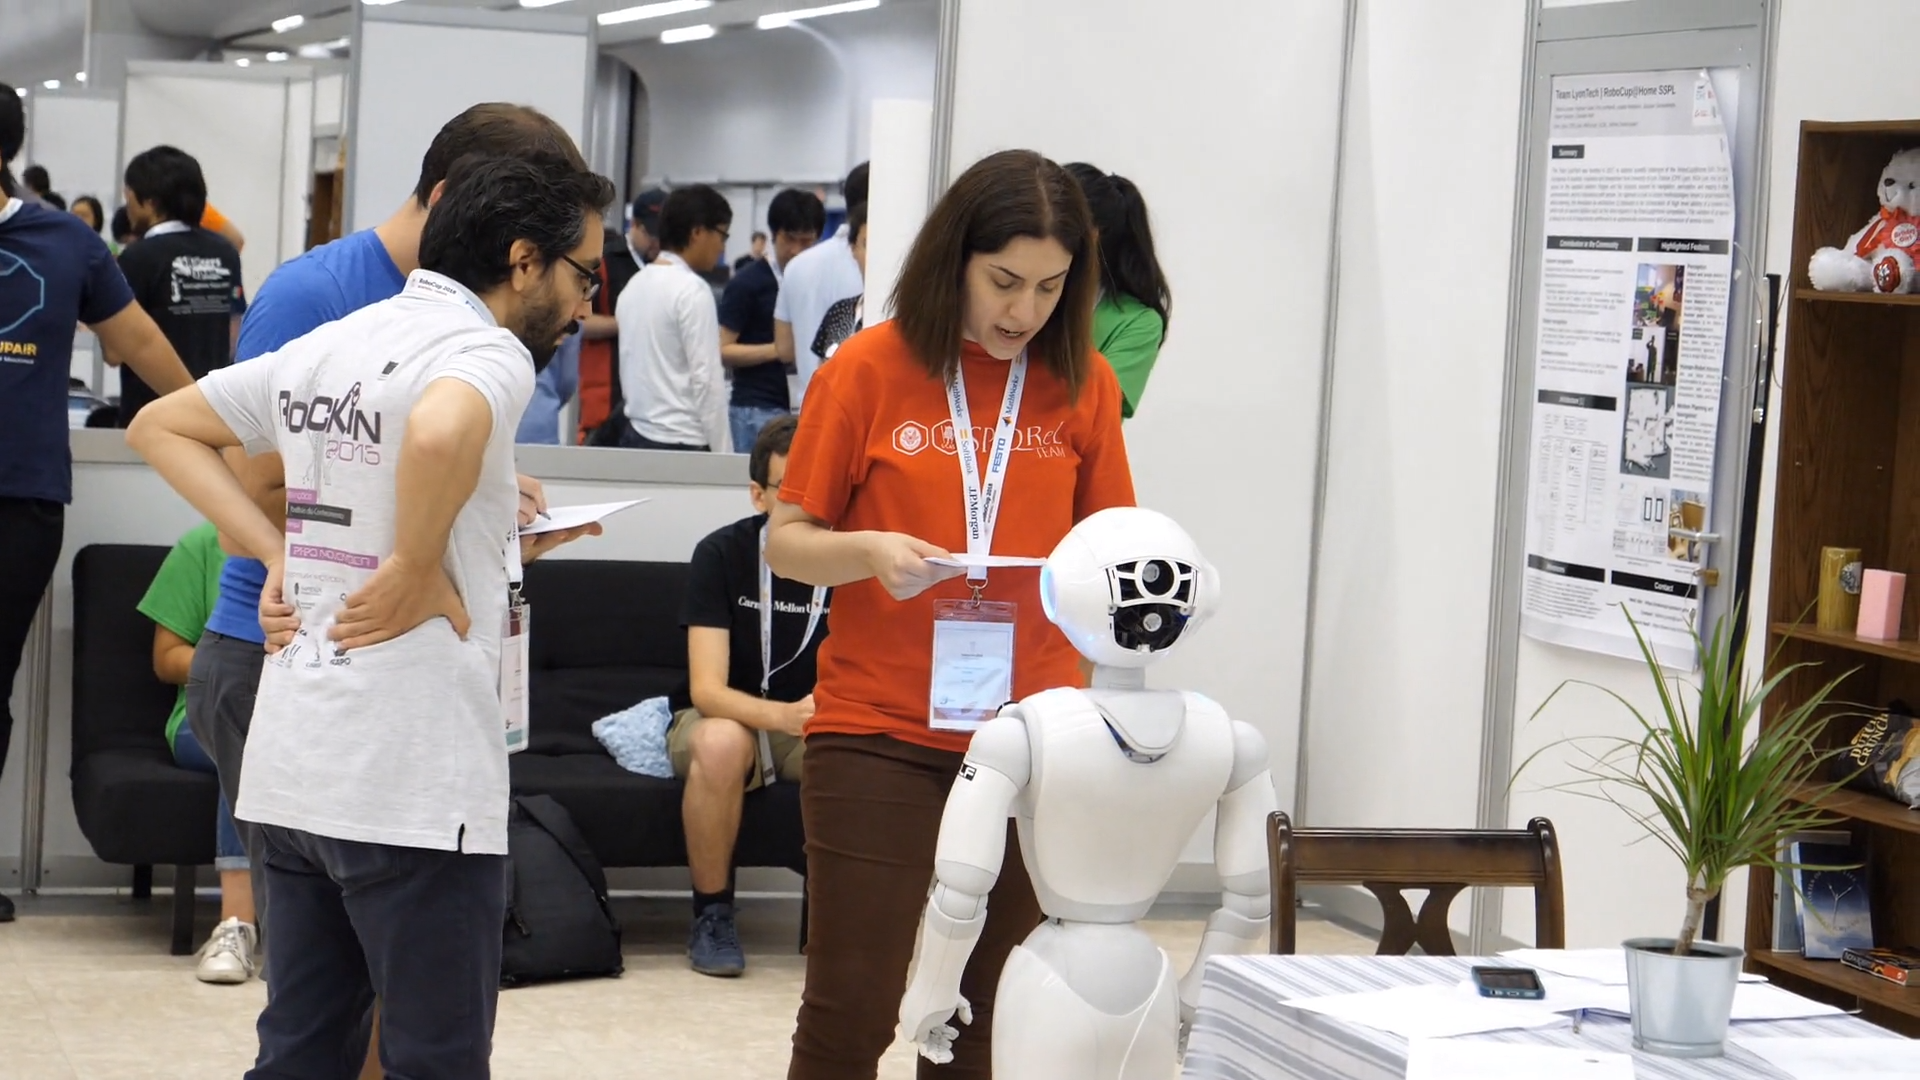
\includegraphics[width=\textwidth]{Bilder/robocup.png}}{Bilder/robocup.mp4}
	\end{frame}
	
	\begin{frame}{Robocup}
		
		\begin{alertblock}{What are requirements for a robot regarding speech recognition? What is nice to have? What would be the optimum?}
			\pause
			\begin{itemize}
				\item[-] first point
				\item[-] second point
				\item[-] third point
			\end{itemize}
		\end{alertblock}
		
	\end{frame}
	
	
	\begin{frame}{Requirements}
		content...
	\end{frame}
	
	
	\begin{frame}{Additional Thoughts}
		content...\\
		was ist eigentlich möglich, welche infos kann man zusätzlich generieren?
	\end{frame}

	\begin{frame}{Evaluation of existing solutions}
		content...
	\end{frame}
	
	\begin{frame}{Foray: Latency vs Signal Integrity}
		content...
	\end{frame}
	
	\begin{frame}{Evaluation of existing solutions II}
		content...
	\end{frame}
	
	
	
	
	
	

	\section{Pipeline}
	
	\begin{frame}{Idea}
		content...
	\end{frame}
	
	\begin{frame}{Architecture}
		content...
		% TODO: diagram
	\end{frame}
	
	\begin{frame}{Interfaces}
		content...
		% TODO: diagram
	\end{frame}
	
	
	
	
	
	
	
	
	\section{Current State}
	\begin{frame}{Progress}
		content...
		https://github.com/Slothologist/rfeldhans-MA-master/projects/1
	\end{frame}
	
	
	
	
	
	
	
	
	
	\section{Evaluation}
	
	\begin{frame}{Robocup Speechrec Task}
		content...
		% TODO: diagram
	\end{frame}
	
	\begin{frame}{Fusion Test}
		content...
		% TODO: diagram
	\end{frame}
	
	\begin{frame}{Dataset Evaluation}
		content...
	\end{frame}
	
	
	
	
	
	\section{Demo}
	
	
	
	
	
	\begin{frame}{}
		\begin{alertblock}{Thanks for your Attention!}
		\end{alertblock}
	\end{frame}
	
	\begin{frame}{}
		\begin{alertblock}{Discussion}
		\end{alertblock}
	\end{frame}
	
\end{document}
	
	
	